\chapter{Slides}
\section{Lecture 1}
The key building blocks of OS
\begin{itemize}
    \item Process 
    \item Threads, Concurrency, Scheduling, Coordination
    \item Address space
    \item Protection, Isolation, Sharing , Security
    \item Communication, Protocols
    \item Persistent storage, Transaction, Consistency, Resilience
    \item Interfaces all devices
\end{itemize}

\begin{figure}
    \centering
    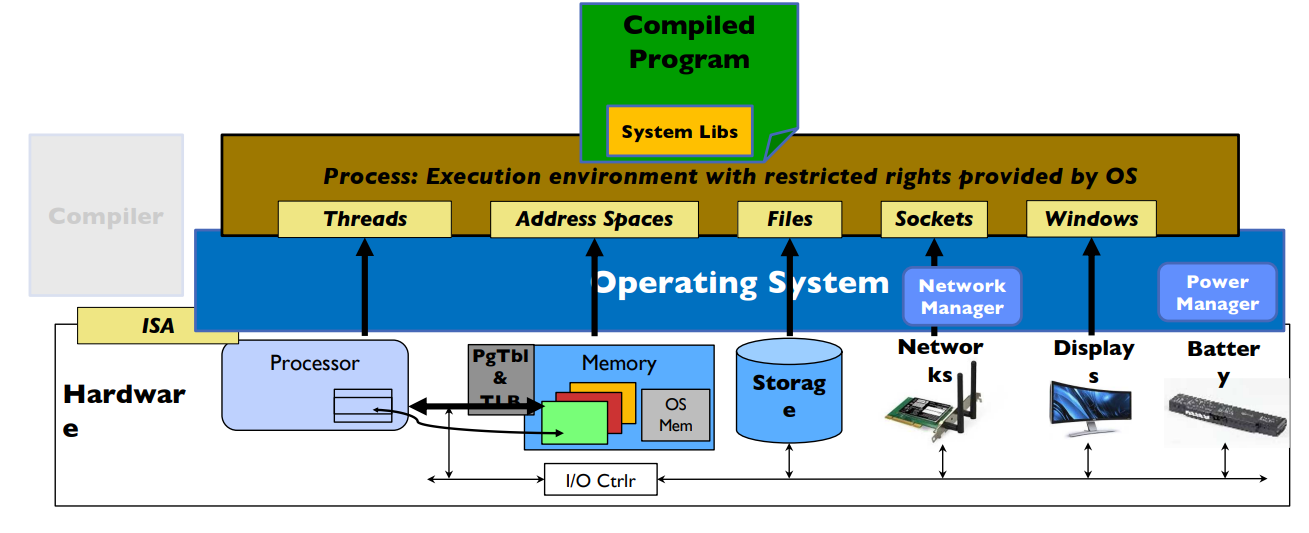
\includegraphics[width = 0.9\textwidth]{Chapters/graphics/OSAbstraction.png}
\end{figure}

\section{Lecture 2}
\subsection{Thread}
A single unit execution context 
\begin{itemize}
    \item It has program counter (PC), registers, execution flags, stack, and memory state
    \item A thread executes on a processor when it is \underline{resident} in the processor's register.
    \item A thread is suspended when its state is not load into processor.
    \item When a thread is not running it's saved in the memory called \underline{thread control unit (TCB)}. 
    \item TCB is saved in kernel.
\end{itemize}

\subsection{Address space}
The set of accessible address and the state associated with them.

\subsection{}
An operating system must 
\begin{itemize}
    \item protect itself from user programs.
    \item be reliable.
    \item be secure.
    \item ensure privacy.
    \item ensure fairness.
    \item protect programs from one another.
    \item prevent threads owned by one program to impact other
\end{itemize}
\subsection{Simple protection: Base and Bound (B\&B)}
sets lower and upperbound for a program to access.

\subsection{Process}
execution enviroment with restricted access. 
\begin{itemize}
    \item (Protected) address space with one or more threads
    \item owns memory
    \item has file descriptors, file system context
    \item encapsulate one or more therad sharing process resources.
\end{itemize}

\subsection{Dual mode}
\begin{enumerate}
    \item Kernel mode (superivor)
    \item User mode
\end{enumerate}